\chapter{Scattering, Mandelstam Variables, and the Open-String Picture}

This lecture begins with a brief return to fermionic strings, but only in order to clear the stage. The real subject is scattering: how a theory takes incoming particles, passes them through an interaction region, and predicts the amplitudes for what comes out. From there the discussion narrows to relativistic kinematics, broadens into the puzzle of channel symmetry, and then deliberately rewinds to the string picture that produces the Veneziano amplitude. The whole chapter has a very definite rhythm: first reduce the kinematics to invariant data, then see why naive point-particle diagrams are not enough, and finally watch the string mechanism rebuild the answer from harmonic oscillators.

\section{From Fermionic Strings Back to Scattering}

Fermionic strings had been part of the subject almost from the beginning. Their role, as Susskind reminds us at the start, is very simple to state: they give us fermions, they remove the tachyons, and they reduce the critical dimension from twenty-six to ten. That still leaves the extra dimensions, but he immediately refuses to be diverted. Compactification is important, and it will come later; for the moment he wants to talk about scattering.

This is a pragmatic turn, and deliberately so. Elementary particle physics has always been driven by scattering experiments, not because scattering is the most profound phenomenon in nature, but because it is what experiment can most reliably access. We send particles in, observe what comes out, and try to reconstruct what happened inside the collision. So the natural question for a theorist is not simply, ``what particles does the theory contain?'' It is: if this is my theory of particles, what scattering amplitudes does it predict?

\section{Four-Momentum, Mass Shell, and the All-Incoming Trick}

To answer that question we first need a language for the kinematics. Susskind starts with the simplest black-box picture: particles go in, something happens in an interaction region, and particles come out. He even changes the usual board convention and draws time horizontally for the evening. A scattering amplitude is then the complex number whose squared magnitude gives the probability for a specified process.

\begin{figure}[htbp]
\centering

\includegraphics[width=0.72\textwidth]{lecture_06_figure_02.png}

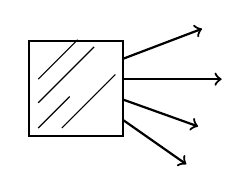
\begin{tikzpicture}[scale=1.0]
\draw[thick] (0,0) rectangle (1.2,1.2);
\draw (0.12,0.10) -- (0.52,0.50);
\draw (0.12,0.42) -- (0.83,1.13);
\draw (0.12,0.72) -- (0.62,1.22);
\draw (0.42,0.10) -- (1.10,0.78);
\draw[->,thick] (1.2,0.98) -- (2.2,1.36);
\draw[->,thick] (1.2,0.72) -- (2.45,0.72);
\draw[->,thick] (1.2,0.46) -- (2.15,0.12);
\draw[->,thick] (1.2,0.20) -- (2.00,-0.36);
\end{tikzpicture}
\caption{Scattering sketch and the start of four-momentum notation. The screenshot preserves the black-box board layout and the transition into new notation; the TikZ redraw keeps only the secure geometric content of the scattering sketch.}
\end{figure}

Each particle carries a relativistic four-momentum,
\begin{equation}
K^\mu=(K^0,\vec K),
\end{equation}
where \(K^0\) is the energy and \(\vec K\) is the spatial momentum. In the lecture the relativistic square is written in the mostly-minus convention
\begin{equation}
K^2 \equiv \vec K^{\,2}-(K^0)^2.
\end{equation}
Starting from the standard dispersion relation
\begin{equation}
E^2=\vec p^{\,2}+m^2,
\end{equation}
he rewrites it as
\begin{equation}
E^2-\vec p^{\,2}=m^2,
\end{equation}
and then flips the sign so that it matches long-standing particle-physics convention,
\begin{equation}
\vec p^{\,2}-E^2=-m^2.
\end{equation}
In terms of \(K^\mu\), that same statement is simply
\begin{equation}
K^2=-m^2.
\end{equation}
This is the first invariant constraint on a particle: one does not vary \(K^2\); rather, one varies the spatial momentum and the energy adjusts so that the mass shell is maintained.

For a \(2\to2\) process the incoming momenta may be called \(K_1\) and \(K_2\), and the outgoing momenta \(Q_3\) and \(Q_4\). Then energy-momentum conservation is
\begin{equation}
K_1+K_2=Q_3+Q_4.
\end{equation}
Susskind then introduces the standard but extremely useful trick of treating all momenta as incoming. One first rewrites conservation as
\begin{equation}
K_1+K_2-Q_3-Q_4=0,
\end{equation}
and then defines
\begin{equation}
K_3=-Q_3,\qquad K_4=-Q_4.
\end{equation}
With that relabeling,
\begin{equation}
K_1+K_2+K_3+K_4=0.
\end{equation}
This is only a bookkeeping device, but it is a very good one. It makes the kinematics symmetric in the four external legs, and because squaring a momentum is unchanged by a sign flip, each leg still satisfies the same mass-shell condition.

Now we can say what the theorist wants. The amplitude is some function
\begin{equation}
A=A(K_1,K_2,K_3,K_4),
\end{equation}
but of course this notation is misleading. It looks as if \(A\) depends on sixteen components, whereas most of that information is redundant.

\section{Center-of-Mass Kinematics and Mandelstam Variables}

Susskind pauses at this point and asks how many independent variables a \(2\to2\) amplitude really depends on. Naively there are four four-vectors, so sixteen components. But momentum conservation already imposes four conditions, and each external leg is on shell. More importantly, one can go to a much better frame.

First move to the center-of-mass frame, where the incoming spatial momenta are equal and opposite. Then rotate the axes so that the collision takes place along a chosen direction. Once that has been done, and once we simplify further by taking all external particles to have the same mass, the initial state depends only on the total center-of-mass energy. The final state must have the same total energy and equal-and-opposite outgoing momenta. What is left for the scattering to know about is only the deflection angle. So the amplitude really depends on just two physical quantities:
\begin{equation}
E_{\mathrm{cm}},\qquad \theta.
\end{equation}

But we do not want quantities that are tied to one frame. We want relativistic invariants. The natural ones are the Mandelstam variables, defined here in a convention consistent with the lecture's choice of sign for \(K^2\):
\begin{equation}
(K_1+K_2)^2=-s,\qquad (K_1+K_3)^2=-t,\qquad (K_1+K_4)^2=-u.
\end{equation}
These are the Mandelstam variables. Susskind remarks on their beautiful symmetric definition, and that symmetry is already part of the story.

The meaning of \(s\) is immediate. In the center-of-mass frame the incoming spatial momenta cancel, so
\begin{align}
(K_1+K_2)^2
&=(\vec K_1+\vec K_2)^2-(K_1^0+K_2^0)^2 \\
&= -E_{\mathrm{cm}}^2.
\end{align}
Therefore
\begin{equation}
s=E_{\mathrm{cm}}^2.
\end{equation}
This is the square of the total energy in the center-of-mass frame.

The meaning of \(t\) is different. Because \(K_3=-Q_3\), we have
\begin{equation}
(K_1+K_3)^2=(K_1-Q_3)^2.
\end{equation}
So \(t\) is the momentum transfer from particle \(1\) to particle \(3\). In the center-of-mass frame, for equal masses and fixed incoming spatial momentum \(|\vec p|\), the clean reconstructed relations are
\begin{equation}
-t = 2|\vec p|^2(1-\cos\theta),\qquad -u = 2|\vec p|^2(1+\cos\theta).
\end{equation}
The transcript is verbally messy on the exact prefactors, but the important physics is clear and reliable: \(t\) and \(u\) know about the scattering angle, whereas \(s\) knows only about the collision energy.

\subsection{Question \& Answer}

Question. If the process really depends only on energy and scattering angle, why do we suddenly introduce three quantities \(s\), \(t\), and \(u\)?

Answer. Because the three Mandelstam variables are not independent. The symmetry of the notation is greater than the number of physical degrees of freedom. Using
\begin{equation}
K_1+K_2+K_3+K_4=0
\end{equation}
together with the on-shell conditions \(K_i^2=-m^2\) for equal external masses, one finds
\begin{equation}
s+t+u=4m^2.
\end{equation}
This is the cleaned form of the constraint that Susskind refers to on the fly. So we have three beautifully symmetric invariants, but only two independent combinations of them, exactly as the center-of-mass analysis demanded.

\section{Channel Diagrams and Simple Pole Amplitudes}

Now that the kinematic variables are in place, Susskind turns to simple Feynman diagrams and asks what kind of amplitudes they give. The first is the direct process: particles \(1\) and \(2\) come together, form an intermediate state of mass \(M\), and then that state decays into \(3\) and \(4\). This is the \(s\)-channel, or direct channel, and its amplitude has the characteristic form
\begin{equation}
A_s \sim \frac{g^2}{s-M^2}.
\end{equation}
The two factors of \(g\) come from the two vertices, and the denominator is the propagator of the intermediate particle.

\begin{figure}[htbp]
\centering

\includegraphics[width=0.62\textwidth]{lecture_06_figure_03.png}

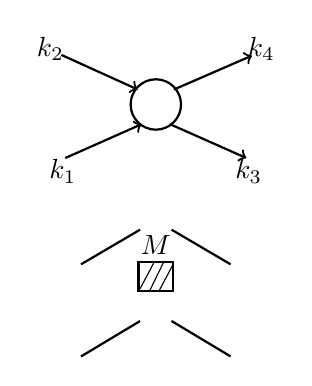
\begin{tikzpicture}[scale=1.0]
\draw[thick] (0,1.85) circle (0.32);
\draw[->,thick] (-1.20,2.48) -- (-0.23,2.04);
\draw[->,thick] (-1.15,1.17) -- (-0.18,1.60);
\draw[->,thick] (0.23,2.04) -- (1.22,2.47);
\draw[->,thick] (0.18,1.60) -- (1.15,1.17);
\node at (-1.34,2.56) {$k_2$};
\node at (-1.18,1.00) {$k_1$};
\node at (1.34,2.56) {$k_4$};
\node at (1.18,1.00) {$k_3$};

\draw[thick] (-0.95,-0.18) -- (-0.20,0.26);
\draw[thick] (-0.95,-1.35) -- (-0.20,-0.90);
\draw[thick] (0.20,0.26) -- (0.95,-0.18);
\draw[thick] (0.20,-0.90) -- (0.95,-1.35);
\draw[thick] (-0.22,-0.52) rectangle (0.22,-0.15);
\draw (-0.20,-0.49) -- (-0.02,-0.15);
\draw (-0.08,-0.52) -- (0.10,-0.15);
\draw (0.04,-0.52) -- (0.22,-0.18);
\node at (0,0.06) {$M$};
\end{tikzpicture}
\caption{Alternate channel diagram with intermediate mass \(M\). The screenshot preserves the two-tier blackboard layout; the redraw stabilizes the geometry and the momentum labels without using the cropped right-edge writing to fix signs.}
\end{figure}

There is then a second diagram, obtained by turning the picture sideways in the sense of the invariants, so that the relevant quantity is \(t\) rather than \(s\). Its amplitude is
\begin{equation}
A_t \sim \frac{g^2}{t-M^2}.
\end{equation}
This is the \(t\)-channel, or crossed channel. One can also imagine a third possibility,
\begin{equation}
A_u \sim \frac{g^2}{u-M^2},
\end{equation}
although Susskind explicitly declines to draw it carefully on the board because crossed lines are annoying to draw and add nothing essential at this point.

The lecture pauses here to interpret the two channel pictures physically. The \(s\)-channel amplitude depends only on the center-of-mass energy. It does not know about the scattering angle. In that sense every deflection angle is equally probable: the incoming particles form a compound state, and when that state decays it has forgotten the direction from which the particles originally came. The direct channel is therefore angle-blind at this crude level.

The \(t\)-channel is different. Since \(t\) depends on the momentum transfer, it depends on the scattering angle. In fact, because small momentum transfer means small deflection angle, this channel favors small-angle scattering. The direct and crossed channels are therefore not only algebraically different; they describe genuinely different kinds of physical processes.

\section{The Veneziano Puzzle}

At this point Susskind takes a historical step back. Formulas like
\begin{equation}
\frac{g^2}{s-M^2}
\end{equation}
are too simple to describe the scattering of mesons. The reason is that when two mesons collide they can produce not just one intermediate particle, but whole towers of excited states with different masses and angular momenta. One therefore tries, at first, to repair the formulas by adding more and more channel contributions: more poles in the \(s\)-channel, more in the \(t\)-channel, and in principle also in the \(u\)-channel.

Then comes the surprise. Instead of a sum of separate channel expansions, a single compact formula was discovered which had the right features of both at once. Susskind writes it partly for historical beauty and partly to set the puzzle as sharply as possible. In canonical modern notation it is
\begin{equation}
A_{\mathrm V}(s,t)\propto \frac{\Gamma(-s)\Gamma(-t)}{\Gamma(-s-t)}.
\end{equation}
He only pauses long enough to remind us what the gamma function is doing: it is the analytic continuation of the factorial, with \(\Gamma(n)=(n-1)!\) at positive integers.

What matters here is not gamma-function technology, but the interpretation. The Veneziano amplitude looks like a sum over infinitely many resonances in the \(s\)-channel. But because it is symmetric in \(s\) and \(t\), it also looks like a sum over infinitely many exchanges in the crossed channel. And these are not two terms to be added. It is the same single function being read in two different ways.

\subsection{Question \& Answer}

Question. How can one symmetric amplitude replace separate \(s\)-channel and \(t\)-channel sums without adding them by hand?

Answer. That is the whole historical puzzle. Prior to this, one would have expected to write down one contribution for direct production and another for exchange, and then add them. The Veneziano amplitude does something stranger: it already contains the analytic features of both channels in one object. The lecture now turns exactly to the question that this raises: what physical mechanism could possibly produce an amplitude of that sort?

\section{Open Strings, Worldsheets, and the String Wave Equation}

Susskind then explicitly rewinds the story. Instead of dwelling on the formula, he asks what sort of microscopic picture could give rise to it. The answer is the open string.

An open string comes with a parameter \(\sigma\) running from one endpoint to the other,
\begin{equation}
0\leq \sigma \leq \pi.
\end{equation}
This is not an ordinary spatial coordinate in spacetime. It is simply a label along the string. The string itself moves through spacetime and, as it moves, sweeps out a two-dimensional surface.

\begin{figure}[htbp]
\centering

\includegraphics[width=0.78\textwidth]{lecture_06_figure_04.png}

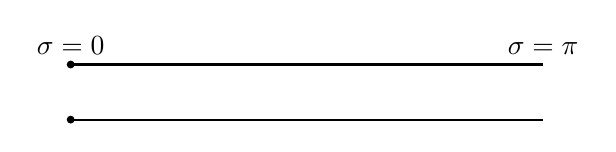
\begin{tikzpicture}[scale=1.0]
\draw[thick] (0,0.45) -- (6.0,0.45);
\draw[thick] (0,-0.25) -- (6.0,-0.25);
\fill (0,0.45) circle (0.05);
\fill (0,-0.25) circle (0.05);
\node[above] at (0,0.45) {$\sigma=0$};
\node[above] at (6.0,0.45) {$\sigma=\pi$};
\end{tikzpicture}
\caption{Open-string parameter interval and endpoint labeling. The board shot records the way the interval is introduced graphically before the notation is fully stabilized; the redraw supplies the endpoint labels stated clearly in the lecture.}
\end{figure}

The old world line of a point particle becomes a worldsheet. Each point on that worldsheet is labeled by two parameters, \(\sigma\) and \(\tau\): \(\sigma\) tells us where we are along the string, and \(\tau\) is the worldsheet time. The string embedding in spacetime is described by \(X(\sigma,\tau)\); the blackboard writes simply \(X\), suppressing the spacetime index. Its equation of motion is the ordinary wave equation on the strip,
\begin{equation}
\frac{\partial^2 X}{\partial \tau^2}-\frac{\partial^2 X}{\partial \sigma^2}=0.
\end{equation}

\begin{figure}[htbp]
\centering

\includegraphics[width=0.62\textwidth]{lecture_06_figure_05.png}
\caption{Worldsheet wave equation for the string coordinate. Here the board equation is fully legible, so the notes preserve the same uppercase \(X\) while typesetting it cleanly.}
\end{figure}

At this point the lecture becomes intentionally pedestrian. Rather than launching into a polished continuum derivation, Susskind reduces the string to something we already understand: a large collection of mass points connected by springs. Then the worldsheet becomes a dense family of world lines, and the dynamics reduces to coupled harmonic oscillators. That is the strategic move. String theory becomes calculable not by magic, but because harmonic oscillators are calculable.

\section{Two Strings Coalesce, Evolve, and Re-Separate}

Now comes the constructive part of the lecture. We begin with two incoming open strings, each approximated by a chain of \(n\) constituents. The first string is described by coordinates \(x_1,\dots,x_n\), the second by \(x_{n+1},\dots,x_{2n}\). For the first chain the center-of-mass position is
\begin{equation}
X_{\mathrm{cm}}^{(1)}=\frac{x_1+\cdots+x_n}{n},
\end{equation}
and for the second,
\begin{equation}
X_{\mathrm{cm}}^{(2)}=\frac{x_{n+1}+\cdots+x_{2n}}{n}.
\end{equation}

Because the first incoming string carries momentum \(k_1\), its wavefunction contains the plane-wave factor \(e^{ik_1\cdot X_{\mathrm{cm}}^{(1)}}\). The rest of the wavefunction depends only on relative positions along the chain and describes the internal ground state of the oscillators. Writing that ground-state factor as \(\psi_0\), the two incoming strings are represented schematically by
\begin{align}
\Psi_1 &= e^{ik_1\cdot X_{\mathrm{cm}}^{(1)}}\,\psi_0(x_1,\dots,x_n),\\
\Psi_2 &= e^{ik_2\cdot X_{\mathrm{cm}}^{(2)}}\,\psi_0(x_{n+1},\dots,x_{2n}).
\end{align}
Since the two strings are initially separate systems, the combined incoming state is their product,
\begin{equation}
\Psi_{\mathrm{in}}=\Psi_1\Psi_2.
\end{equation}
This is one of those moments where Susskind slows down to say something very elementary but essential: separate quantum systems combine by multiplication of wavefunctions.

The next step is to ask for the amplitude that the endpoints of the two strings touch. In the discrete description that means imposing the condition
\begin{equation}
x_n=x_{n+1}.
\end{equation}
We do not set this from the start; rather, we look inside the incoming wavefunction for the part in which these two endpoint coordinates coincide. Once that happens, the two strings are allowed to coalesce into a single chain. In the spring-and-mass picture, one simply says that a new spring appears between the last constituent of the first string and the first constituent of the second.

After that, the joined object evolves for some duration, which the lecture again calls \(\tau\). In cleaned notation we may represent that evolution by
\begin{equation}
\Psi(\tau)=e^{-iH\tau}\Psi(0),
\end{equation}
where \(H\) is the Hamiltonian of the single longer chain. The transcript is not stable on the sign convention in the exponential, so the expression above should be read as the standard Schr\"odinger form, not as a claim about the precise sign on the blackboard.

The last step is to project the evolved joined state onto a final state consisting again of two separated strings carrying momenta \(k_3\) and \(k_4\). The logical order matters, and Susskind keeps repeating it:
\begin{enumerate}
\item begin with two incoming string ground states,
\item multiply them to make the initial composite wavefunction,
\item constrain the endpoints to be at the same point,
\item evolve the joined string as a single dynamical system,
\item project onto a final two-string state.
\end{enumerate}
That gives the amplitude for joining, propagating for a time \(\tau\), and splitting again.

\subsection{Question \& Answer}

Question. Why do we integrate over the intermediate time \(\tau\), and what are we summing over?

Answer. We integrate because the lifetime of the joined string is not fixed. Feynman's rule is to sum over all possibilities. In this setup the remaining continuous parameter is precisely the time for which the two strings stay fused before they separate again. So the sum over histories becomes an integral over all allowed \(\tau\).

The lecture then writes down the answer in a form that is corrected live as it is being discussed. Cleaning the signs into a consistent convention gives a representative integrand of the form
\begin{equation}
A(s,t)\propto \int_0^\infty d\tau\, e^{-\tau(s+1)}\bigl(1-e^{-\tau}\bigr)^{-t-1}.
\end{equation}
What matters is not the precise on-the-fly blackboard bookkeeping of every minus sign, but the structure: one factor carries the \(s\)-dependence, another carries the \(t\)-dependence, and the amplitude is obtained by integrating over the duration of the joined phase.

Now comes the surprise. Let
\begin{equation}
z=e^{-\tau}.
\end{equation}
Then \(d z = -e^{-\tau}d\tau\), the range \(\tau\in[0,\infty)\) becomes \(z\in[1,0]\), and after reversing the limits one obtains
\begin{equation}
A(s,t)\propto \int_0^1 z^{-s-1}(1-z)^{-t-1}\,dz.
\end{equation}
This is the Euler beta function,
\begin{equation}
A(s,t)\propto B(-s,-t)=\frac{\Gamma(-s)\Gamma(-t)}{\Gamma(-s-t)}.
\end{equation}
So the joining-and-splitting of two open strings reproduces the Veneziano amplitude.

The symmetry that looked so mysterious before is now visible directly in the integral. Under the change of variables \(z\mapsto 1-z\),
\begin{align}
A(s,t)
&\propto \int_0^1 z^{-s-1}(1-z)^{-t-1}\,dz \\
&= \int_0^1 z^{-t-1}(1-z)^{-s-1}\,dz \\
&= A(t,s).
\end{align}
The astonishing thing, as Susskind stresses, is that the construction began in a way that looked very asymmetric between collision energy and momentum transfer. Yet the final answer is completely symmetric between \(s\) and \(t\). The deeper reason is deferred to the next lecture: conformal symmetry on the worldsheet, the symmetry that lets one stretch the sheet like Turkish taffy and reinterpret the same process in different channel pictures.

\subsection{Question \& Answer}

Question. In the discrete string picture, when two endpoint constituents meet, why do two disappear rather than one?

Answer. This comes up as a late but genuine consistency check. The right way to think about it is that the touching endpoint of one chain and the touching endpoint of the other annihilate as a pair. The new spring then connects the next surviving constituents. In that discrete language one has \(2n-2\) constituents rather than \(2n-1\). For the continuum limit the difference is negligible, but conceptually it matters: one must not lose an odd number of fermionic degrees of freedom.

Susskind then adds three closing clarifications. First, the same basic calculation was originally done for the bosonic string and changes only slightly for superstrings. Second, the analogous process for closed strings is very similar: two closed strings join into one closed string, propagate, and then split again. Third, and historically most important, once these amplitudes were calculated for the spin-one and spin-two states in the string spectrum, they behaved not like generic scalar amplitudes but like the distinctive amplitudes of photons and gravitons. That was one of the sharp signals that string theory had stumbled into something much deeper than a phenomenological model of hadrons.

\section{Summary}

The lecture unfolds in a very deliberate sequence. We begin with ordinary relativistic scattering, define four-momentum and the mass shell, and use the all-incoming convention to put the kinematics into a symmetric form. We then strip a \(2\to2\) process down to its invariant content and package that content into the Mandelstam variables. From there the direct and crossed channels acquire a clear physical meaning: one forms a compound state that forgets its incident direction, the other transmits momentum and remembers the scattering angle.

The real surprise comes when those two channel pictures are no longer added separately, but are replaced by the single Veneziano amplitude. The second half of the lecture then rewinds from that formula to the mechanism behind it: two strings join, evolve as one, and split again. The resulting integral is the Euler beta function, and therefore the Veneziano amplitude itself. What still remains to be explained is why the answer is symmetric between \(s\) and \(t\). That deeper answer lies in conformal symmetry on the worldsheet, and it is left, quite deliberately, for next time.